\begin{figure}[h]
  \begin{subfigure}{.5\textwidth}
    \centering
    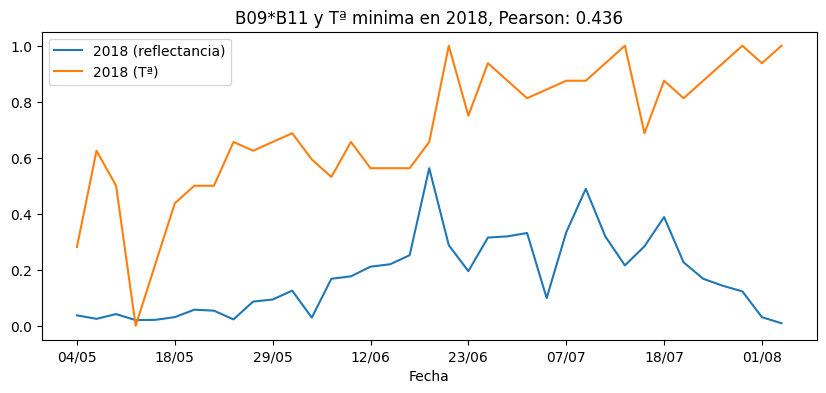
\includegraphics[width=1\linewidth]{figures/xanyos_Tamin-B9x11/0.png}
    \caption{}
  \end{subfigure}
  \begin{subfigure}{.5\textwidth}
    \centering
    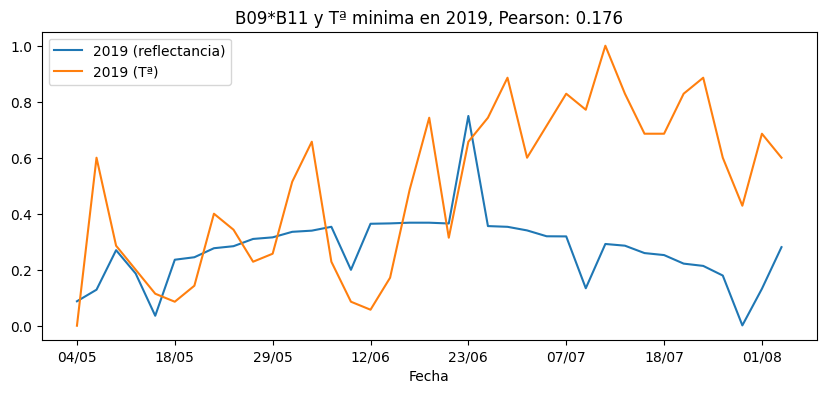
\includegraphics[width=1\linewidth]{figures/xanyos_Tamin-B9x11/1.png}
    \caption{}
  \end{subfigure}
  \begin{subfigure}{.5\textwidth}
    \centering
    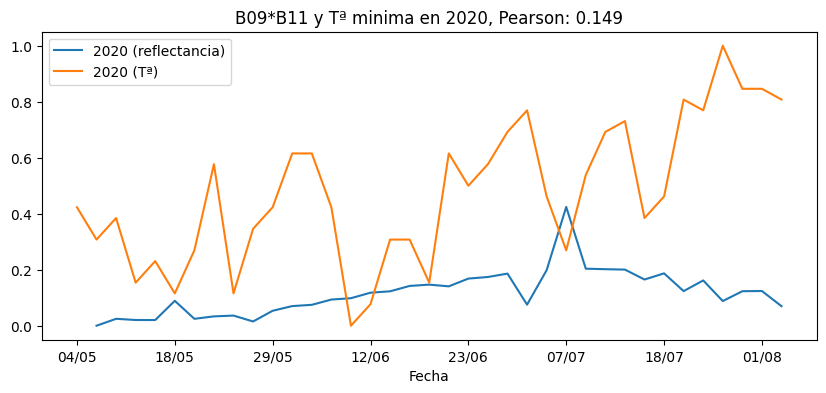
\includegraphics[width=1\linewidth]{figures/xanyos_Tamin-B9x11/2.png}
    \caption{}
  \end{subfigure}
  \begin{subfigure}{.5\textwidth}
    \centering
    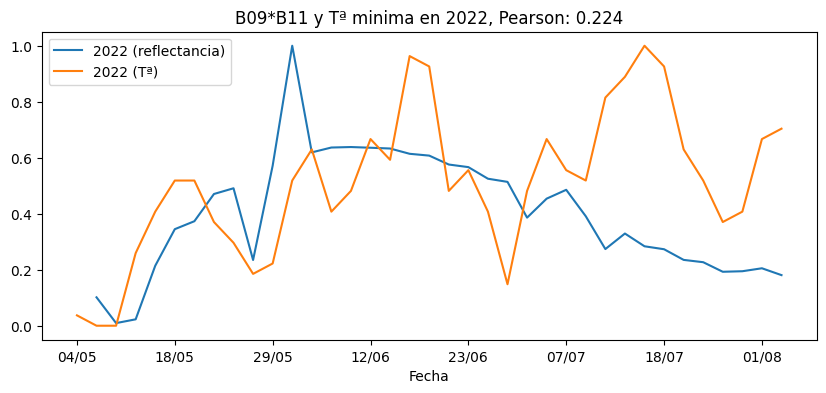
\includegraphics[width=1\linewidth]{figures/xanyos_Tamin-B9x11/3.png}
    \caption{}
  \end{subfigure}
    \caption{Curvas de la Tª mínima junto con la reflectancia de $B_{09}*B_{11}$}
    \label{fig:xanyos_Tamin-B9x11}
\end{figure}